\begin{Def}
A Linear Space is a pair
\[(P,L)\] 
where \(P\) is a set whose elements are called points 
 and \(L\subseteq \mathcal{P}(P)\) a set of subsets of \(P\) called lines such that 
 \begin{Axiom}[I1]
    For \(A,B\in P\) with \(A\neq B\) there exists a unique 
    \(\ell\in L\) such that \(A,B\in \ell\).\label{Axiom:I1} 
    \end{Axiom} 
\begin{Axiom}[I2]For every \(\ell\in L\) there are \(A,B\in \ell\) with \(A\neq B\).
\end{Axiom}
\begin{Axiom}[I3] There are three noncollinear points, i.e. there are 
    \(A,B,C\in P\) such that there is no \(\ell\in L\) with \(A,B,C\in\ell\).
 \end{Axiom}
\end{Def}
\begin{Satz}
Let \[(P,L)\] be a Linear Space. 
If \(\ell,m\in L\) are two distincs lines, then \(\ell\cap m\) has at most one point.
\end{Satz}
\begin{proof} 
Assume there were \(A,B\in \ell\cap m\) with \(A\neq B\).
By \axiomref{Axiom:I1} there is a unique line containing both points \(A,B\). 
But then it follows that \(\ell=m\) which is a contradiction since they were assumed to be distinct.
\end{proof}
\begin{Bsp}
Let \(P=\{A,B,C\}\) and \(L=\{\ell=\{A,B\},m=\{A,C\},n=\{B,C\}\}\). Then 
\((P,L)\) is an Incidence Geometry.
\begin{figure}[H]
    \centering
\begin{tikzpicture}
  % Drei Ecken eines gleichseitigen Dreiecks (auf einem Kreis)
  \node (A) at (90:2)  {$A$}; 
  \node (B) at (210:2) {$B$};
  \node (C) at (330:2) {$C$};

  % Verbindungs-Pfeile
  \draw[-] (A) -- node[left]  {$\ell$} (B);
  \draw[-] (B) -- node[below] {$n$} (C);
  \draw[-] (A) -- node[right] {$m$} (C);
\end{tikzpicture}
\end{figure}
\end{Bsp} 

\begin{Bsp}
    Let \(P,L\) be a linear Space with \(|P|\geq 4\). Let \(A\in P\).
    Then \(P\setminus\{A\},L\setminus\{\ell\mid A\in \ell\}\) ist again a linear space.
    Because let \(B,C\in P\setminus\{A\}\) with \(B\neq C\).
    Then there is a line \(\ell\in L\) with \(C,B\in \ell\). 
\end{Bsp}
\begin{Bsp}
    Let \(M\) be a set with at least \(3\) elements. Then 
    \[(M,\{\{A,B\}\mid A\neq B\in M\})\] is a Linear Space.
\end{Bsp}

\begin{Def}
A Morphism \(f\colon (P,L)\to (P',L')\) of Linear Spaces is a map of sets 
\(f^\#\colon P\to P'\) such that that for every \(\ell\in L\) the set 
\(f^\#(\ell)\subseteq \ell'\) for some \(\ell'\in L\).
A Morphism \(f\colon (P,L)\to (P',L')\) is called Monomorphism, if there is a Morphism
\(g\colon (P,L)\to (P',L')\) such that \(gf=\id\).
\end{Def}
\begin{Bsp}
Let \(P=\{A,B,C,D\}\) be a set of 4 points. 
Let \(L_1=\{\{A,B,C\},\{A,D\},\{B,D\},\{C,D\}\}\) and 
\(L_2=\{\{A,B\},\{A,C\},\{A,D\},\{B,C\},\{B,D\},\{C,D\}\}\). 
Then up to isomorphism \((P,L_1)\) und \((P,L_2)\) are the only Linear Spaces with 4 points
\begin{figure}[H]
    \centering
    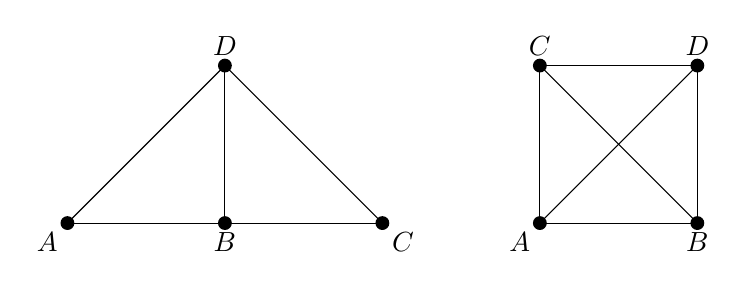
\begin{tikzpicture}
    \coordinate (A) at (-5,0);
    \coordinate (B) at (-3,0);
    \coordinate (C) at (-1,0);
    \coordinate (D) at (-3,2);
    \coordinate (E) at (1,0);
    \coordinate (F) at (3,0);
    \coordinate (G) at (1,2);
    \coordinate (H) at (3,2);

    % Lines
    \draw (A) -- (C);   % {A,B,C}
    \draw (A) -- (D);   % {A,D}
    \draw (B) -- (D);   % {B,D}
    \draw (C) -- (D);   % {C,D}
    \draw (E) -- (F);
    \draw (E) -- (G);
    \draw (E) -- (H);
    \draw (F) -- (G);
    \draw (F) -- (H);
    \draw (G) -- (H);

    % Points
    \fill (A) circle (2.5pt) node[below left] {$A$};
    \fill (B) circle (2.5pt) node[below] {$B$};
    \fill (C) circle (2.5pt) node[below right] {$C$};
    \fill (D) circle (2.5pt) node[above] {$D$};
    \fill (E) circle (2.5pt) node[below left] {$A$};
    \fill (F) circle (2.5pt) node[below] {$B$};
    \fill (G) circle (2.5pt) node[above] {$C$};
    \fill (H) circle (2.5pt) node[above] {$D$};
    
    \end{tikzpicture}
    
\end{figure}
\end{Bsp}
\begin{Bsp}
Let \(P\) be a Linear Space. If 
\(|P|\geq 4\) then there is a point \(A\in P\) such that there are three non-collnear points 
in \(P\setminus\{A\}\).
Then let \(P'=P\setminus\{a\}\) and \(L'=\{\ell\setminus\{A\}\mid \ell\in L, |\ell\setminus\{A\}\geq 2|\).
Then \((P',L')\to (P,L)\) is a Monomorphism.

\end{Bsp}
\begin{Satz}\label{Satz:PointOnTwoLine}
Let \((P,L)\) be a Linear Space.
Every point \(A\) lies on at least two distinct lines.
\end{Satz}
\begin{proof}
By \axiomref{Axiom:I1}  and \axiomref{Axiom:I3} there is a line \(\ell\) with \(A\in \ell\). 
and a point \(B\) not on that line.
Then by \axiomref{Axiom:I1} there is a unique line \(\ell'\) with \(A,B\in \ell'\). 
We have \(\ell\neq \ell'\) since \(B\in\ell'\) but \(B\not\in\ell'\).
\end{proof}
\begin{Satz}
Let \((P,L)\) be a finite Linear Space. Then 
\(|P|\leq |L|\).
\end{Satz}
\begin{proof}
Let \(P=\{p_1,\dots,p_n\}\) and \(L=\{\ell_1,\dots,\ell_m\}\). 
Define the \(n\times m\) Matrix \(A\) by 
\[A_{ij}=\begin{cases} 1 & p_i\in \ell_j\\
    0 & p_i\not\in \ell_j
\end{cases}\] 
Then \((AA^T)_{ij}\) is the number of lanes both containing \(p_i\) and \(p_j\).
if \(i\neq j\) then by \axiomref{Axiom:I1} we have \((AA^T)_{ij}=1\) and 
\((AA^T)_{ii}\) is the number \(r_i\) of lines containig \(p_i\). 
Then 
\[AA^T=J+diag(r_1-1,\dots,r_n-1)\] where \(J\) has 1 as entry everywhere.
Now by \cref{Satz:PointOnTwoLines} we have \(r_i\geq 2\). 
Thus \(diag(r_1-1,\dots,r_n-1)\) is positive definite and thus 
\(AA^T\) is positive definite.
Then \(n=rank(AA^T)\leq rank(A)\leq m\).
\end{proof}
\begin{Def}
Let \((P,L)\) be a finite Linear Space.
Denote by \(n=|P|\), \(m=|L|\) and for \(\ell\in L\) and \(p\in P\) let 
\[k_\ell=|\ell|\] and \[r_p=|\{\ell'\mid p'\in \ell'\}|\]
\end{Def}
\begin{Satz}
Let \((P,L)\) be a finite Linear Space and \(p\in P\) and \(\ell\in L\). 
If \(p\not\in \ell\) then \(r_p\geq k_\ell\).
\end{Satz}
\begin{proof}
Let \(p\not\in\ell\). 
Then there for every \(p_i\in \ell\) exactly one line 
\(\ell_i\) with \(p,p_i\in \ell_i\). All those lines are distinct otherwise
\(p\in \ell\) would give a contradiction.
Hence the statement follows.
\end{proof}
\begin{Satz}
    Let \((P,L)\) be a finite Linear Space such that 
    \(k_\ell\geq 3\) for all \(\ell\in L\). 
    Then for two lines \(\ell,m\in L\) there is a point 
    \(p\not\in \ell\cup m\).
\end{Satz}
\begin{proof}
    Let wlog \(\ell,m\) be distinct and \(x\in \ell\setminus m\), 
    \(y\in m\setminus \ell\).
    Let \(o\) be the unique line through \(x\) and \(y\).
    Since \(k_o\geq 3\) we can choose \(z\in o\) with \(z\neq x\) and \(z\neq y\).
    If \(z\in\ell\) were true, then \(o\) and \(\ell\) share 
    two points \(z\) and \(x\) making \(o=\ell\) which contradicts \(y\not\in\ell\).
    Similarly \(z\not\in m\) so \(z\not\in\ell\cup m\).
\end{proof}
\begin{Satz}
Let \((P,L)\) be a finite Linear Space.
Then 
\[\sum_{\ell\in L}\binom{k_\ell}{2}=\binom{m}{2}\]
and for \(p\in P\) we have
\[\sum_{p\in \ell}(k_\ell-1)=n-1\]
\end{Satz}
\begin{proof}
    Let \(M=\{\{A,B\}\mid A\neq B\in B\}\). 
    Then \(\binom{n}{2}=|M|\). 
    But also 
    \(M=\coprod_{\ell\in L}\{\{A,B\}\mid A\neq B\in \ll\}\).
    Thus 
    \[|M|=\sum_{\ell\in L}\binom{k_\ell}{2}\] and the first statement follows.
    Similarly,
    \(P\setminus{p}=\coprod_{p\in \ell}\ell\setminus\{p\}\) such that 
    the second statement follows.
\end{proof}






\begin{Satz}
Let \((P,L)\) be a finite Linear Space. Then 
\[\sum_{p\in P}r_p=\sum_{\ell\in L}k_\ell\]
\end{Satz}
\begin{proof}
Let \(P=\{p_1,\dots,p_n\}\) and \(L=\{\ell_1,\dots,\ell_m\}\).
Define the \(n\times m\) Matrix \(A\) by 
\[A_{ij}=\begin{cases} 1 & p_i\in \ell_j\\
    0 & p_i\not\in \ell_j
\end{cases}\] 
\((AA^T)_{ii}=r_{p_i}\) and
\((A^TA)_{jj}=k_{\ell_j}\). 
Thus
\[\sum_{p\in p}r_p=tr(AA^T)=tr(A^TA)=\sum_{\ell\in L}k_\ell.\]
\end{proof}


\begin{Kor}
Assume \((P,L)\) is a finitie Linear Space.

If \(k_\ell=k\) for all \(\ell\in L\) then 
\(r_p=r\) for all \(p\in P\) and in this case 
\[r=\dfrac{|P|-1}{k-1}\] and 
\[|L|=\dfrac{|P|(|P|-1)}{k(k-1)}\]
\end{Kor}
\begin{proof}
Assume \(k=k_\ell\) for all \(\ell\in L\). 
Then for every \(p\in P\) we have
\(r_p(k-1)=|P|-1\) so \[r_pr=\dfrac{|P|-1}{k-1}.\]
And by ??? \[|P|r=|L|k\] such that 
\[|L|=\dfrac{|P|(|P|-1)}{k(k-1)}\]

\end{proof}
\begin{Kor}
Let \((P,L)\) be a finite Linear Space such that \(k_\ell=k\) for all \(\ell\in L\).
Then \(|P|\geq k^2-k_\ell+1\) and equality if \(|P|=|L|\).
\end{Kor}
\begin{proof}
    By ?? we have 
    \[|L|\geq |P|\] and combing with ?? gives 
    \[|P|\leq\dfrac{|P|(|P|-1)}{k(k-1)}\]  
    Solving for \(|P|\) gives the statement.
\end{proof}
\begin{Bsp}
Look at the following Linear Space.
\begin{figure}[H]
    \centering
    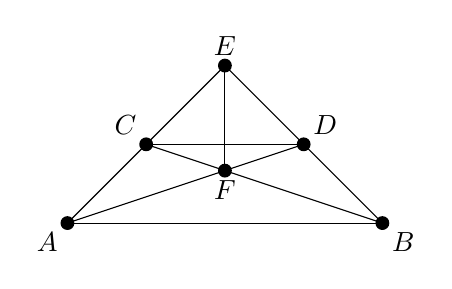
\begin{tikzpicture}
        \coordinate (A) at (-2,0);
        \coordinate (B) at (2,0);
        \coordinate (C) at (-1,1);
        \coordinate (D) at (1,1);
        \coordinate (E) at (0,2);
        \coordinate (F) at (0,0.666);

        \draw (A) -- (B);
        \draw (A) -- (D);
        \draw (A) -- (E);
        \draw (B) -- (C);
        \draw (B) -- (E);
        \draw (C) -- (D); 
        \draw (E) -- (F);

        
    % Points
    \fill (A) circle (2.5pt) node[below left] {$A$};
    \fill (B) circle (2.5pt) node[below right] {$B$};
    \fill (C) circle (2.5pt) node[above left] {$C$};
    \fill (D) circle (2.5pt) node[above right] {$D$};
    \fill (E) circle (2.5pt) node[above] {$E$};
    \fill (F) circle (2.5pt) node[below] {$F$};
    \end{tikzpicture}
\end{figure}
We have \(r_p=3\) for all \(p\in P\) but \(k_\ell\) takes the values 
\(2\) and \(3\).
\end{Bsp}
\begin{Satz}
Assume \((P,L)\) is a finite Linear Space such that \(|P|=|L|\).\\
Then 
\begin{enumerate}
    \item \[r_p=k_\ell\] for every \(p\in P\) and \(\ell\in L\) with 
\(p\not\in \ell\).

\item Every two lines meet in 
at least one point, \(i.e\) \(\ell\cap m\neq\empty\) for \(\ell,m\in L\).
\end{enumerate}
If futhermore \(k_\ell\geq 3\) for every then 
\[k_\ell=r_p=q+1\] for all \(\ell\in L\) and \(p\in P\) and \[|P|=q^2+q+1\]
\end{Satz}
\begin{proof}
Let \(p\in P\) and \(\ell\in L\) such that 
\(p\not\in\ell\).
Since \(r_p\geq k_\ell\) we have
\[|L|(|P|-k_\ell)\geq |P|(|L|-r_p)\] or equivalently
\[\dfrac{1}{|L|(|P|-k_\ell)}\leq \dfrac{1}{|P|(|L|-r_p)}\]  
Summing over all pairs \((p,\ell)\) with \(p\not\in \ell\) gives on the left hand sinde 
\[\sum_{\ell}\sum_{p\not\in\ell}\dfrac{1}{|L|(|P|-k_\ell)}=\sum_{\ell}\frac{|P|-k_\ell}{|L|(|P|-k_\ell)}=1\] 
and similarly \[\sum_{p}\sum_{\ell\not\ni p}\dfrac{1}{|P|(|L|-r_p)}=1\]. 
Thus every \(\leq\) is an \(=\) such that 
\(r_p=k_\ell\) whenever \(p\not\in\ell\).
Now let \(\ell,m\in L\) be distinct lines and 
\(p\in m\setminus\{\ell\}\).
Then \(r_p=k_\ell\)
But for every \(x\in \ell\) the lines that contain \(p\) and \(x\) are already 
\(k_\ell\) distinct lines through \(p\) so they are all lines through \(p\).
In particular, \(m\) is one of them and thus
\(\ell\cap m\neq \emptyset\).
        Now let furthermore \(k_\ell\geq 3\).
        By ?? there is a point \(p\not\in \ell\cup m\).
        Therefore \[k_\ell=r_p=k_m\] and thus 
        \(k_\ell=R_p=q+1\) for all \(\ell\in L\) and \(p\in P\)
        By?? we have 
        \[q+1=\frac{|P|-1}{q}\] such that \(|P|=q^2+q+1\).
\end{proof}
\begin{Bsp}[Fano Plane]
The following Linear Space fullfills the assumptions of ???

\begin{figure}[H]
    \centering
    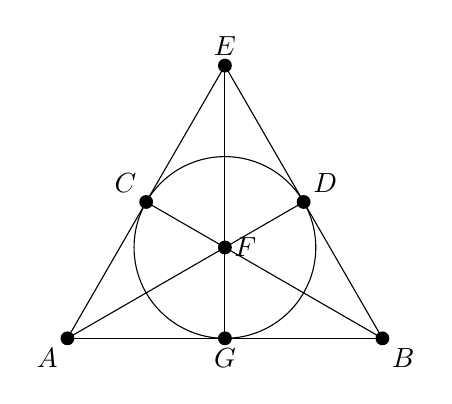
\begin{tikzpicture}
        \coordinate (A) at (-2,0);
        \coordinate (B) at (2,0);
        \coordinate (C) at (-1,1.732);
        \coordinate (D) at (1,1.732);
        \coordinate (E) at (0,3.464);
        \coordinate (F) at (0,1.154);
        \coordinate (G) at (0,0);

        \draw (A) -- (B);
        \draw (A) -- (D);
        \draw (A) -- (E);
        \draw (B) -- (C);
        \draw (B) -- (E);
        \draw (E) -- (G);
        \draw (F) circle[radius=1.154];

        
    % Points
    \fill (A) circle (2.5pt) node[below left] {$A$};
    \fill (B) circle (2.5pt) node[below right] {$B$};
    \fill (C) circle (2.5pt) node[above left] {$C$};
    \fill (D) circle (2.5pt) node[above right] {$D$};
    \fill (E) circle (2.5pt) node[above] {$E$};
    \fill (F) circle (2.5pt) node[right] {$F$};
    \fill (G) circle (2.5pt) node [below] {$G$};
    \end{tikzpicture}
\end{figure}
\end{Bsp}
\begin{Def}[Parallel Lines]
Let \((P,L)\) be a Linear Space.
Then two lines \(\ell,m\in L\) are called parallel, if \(\ell\cap m=\emptyset\) or \(\ell=m\).
\end{Def}
\begin{Bsp}
    The property parallel is not an equivalence relation on \(L\).
    For example
    \begin{figure}[H]
    \centering
    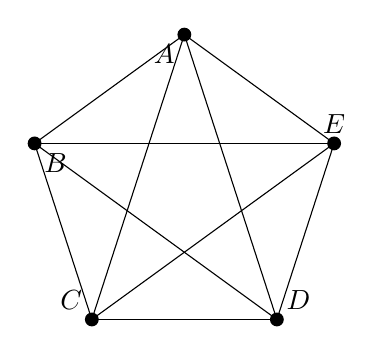
\begin{tikzpicture}
        \coordinate (A) at (0,2);
        \coordinate (B) at (-1.902,0.618);
        \coordinate (C) at (-1.175,-1.618);
        \coordinate (D) at (1.175,-1.618);
        \coordinate (E) at (1.902,0.618);

        \draw (A) -- (B);
        \draw (A) -- (C);
        \draw (A) -- (D);
        \draw (A) -- (E);
        \draw (B) -- (C);
        \draw (B) -- (D);
        \draw (B) -- (E);
        \draw (C) -- (D);
        \draw (C) -- (E);
        \draw (D) -- (E);

        
    % Points
    \fill (A) circle (2.5pt) node[below left] {$A$};
    \fill (B) circle (2.5pt) node[below right] {$B$};
    \fill (C) circle (2.5pt) node[above left] {$C$};
    \fill (D) circle (2.5pt) node[above right] {$D$};
    \fill (E) circle (2.5pt) node[above] {$E$};
    \end{tikzpicture}
\end{figure}

Here \(\overline{AB}\parallel \overline{CD}\) and \( \overline{CD} \parallel \overline{AE}\) aber 
\(\overline{AB}\not\parallel \overline{AE}\) 
\end{Bsp}
\begin{Satz}
Let \((P,L)\) be a Linear Space.
Then it is equivalent:
\begin{enumerate}
\item For every line \(\ell\in L\) and every point \(p\in P\) with \(p\not\in \ell\) there is at most 
one line \(m\in L\) with \(p\in m\) and \(m\parallel \ell\). 
\item Being Parallel is an equivalence relation on \(L\).
\end{enumerate}
\end{Satz}
\begin{proof}
    Assume \((1)\).
    Being parallel is always symmetric and reflexive.
    So assume \(\ell\parallel m\) and \(m\parallel o\).
    if \(p\in \ell\cap o\) then \(p\not\in m\) but since there is at most one line containing \(p\) and 
    being parallel to \(m\) we have that \(o=\ell\) so \(\ell\parallel o\).
    Assume \((2)\) and let \(p\not\in \ell\) be a point.
    Assume there are two lines \(m,o\) through \(p\) with
    \(m\parallel \ell\) and \(o\parallel \ell\). Then \(m\parallel o\) but since they have the point 
    \(p\) in common, they must be equal.
\end{proof}
\begin{Bem}

    We call the Axion 
    \begin{Axiom}(P)
        For every line \(\ell\in L\) and every point \(p\in P\) with \(p\not\in \ell\) there is at most 
one line \(m\in L\) with \(p\in m\) and \(m\parallel \ell\).
    \end{Axiom} the Parallel Axiom. 
    There is a stronger version of this Axiom
    \begin{Axiom}(P')
        For every line \(\ell\in L\) and every point \(p\in P\) with \(p\not\in \ell\) there is exactly 
one line \(m\in L\) with \(p\in m\) and \(m\parallel \ell\).
    \end{Axiom}
\end{Bem}
